%!TEX root = ../memoire.tex

\chapter{Génération automatique de texte}

%%%%%%%%%%%%%%%%%%%%%%%%%%%%%%%%%%%%%%%%%%%%%%%%%%%%%%%
% --------- I N T R O   ---------
%%%%%%%%%%%%%%%%%%%%%%%%%%%%%%%%%%%%%%%%%%%%%%%%%%%%%%%

La \acf{GAT} découle de la branche qu'est le \acf{TAL}. Reiter et Dale  définissent cette branche comme étant un domaine à la croisée des chemins entre l'intelligence artificielle et la linguistique computationnelle \citep{ReiterBuildingNaturalLanguage2000}. L'objectif de la \ac{GAT} est de développer des sytèmes pouvant produire du texte compréhensible en langue naturelle à partir de données (non-linguistiques). Bien que cet objectif soit commun à tous les générateurs de texte, il existe diverses méthodes pour l'achever. La diversité des méthodes est une conséquence directe des divers types d'input possibles (données non-linguistiques, texte et des images \citep{thomason:coling14}) et des diverses approches pour réaliser l'output (à base de patrons, à base de règles, stochastiques \citep{gatt18}).

Toutefois, avant d'entrer dans les détails de la \ac{GAT}, il serait pertinent de présenter l'origine de ces systèmes. À la base, ils ont été conçus pour, entre autre, générer des rapports automatiquement afin de faciliter le travail des êtres humains \citep{ReiterBuildingNaturalLanguage2000}. À ce sujet, Daoust et Lapalme soutiennent que\cite{DaoustJSREALTextRealizer2015} la \ac{GAT} nous permet de générer un résumé d'information provenant d'un input numérique qui est incompréhensible pour un humain. D'ailleurs, en plus de fournir des résumés automatiques, ces systèmes de \ac{GAT} opèrent les tâches sans se fatiguer. Ces tâches automatiées permettent d'éviter des coûts en termes de ressources et de temps. De plus, les textes générés automatiquement n'ont pas besoin d'être lus par une quantité phénomènale de gens pour être considérés utiles. Dès qu'ils remplissent leur fonction auprès d'une poignée de gens, leur raison d'être est justifiée. On est même capable de générer du texte en fonction du lecteur. Ainsi, on pourrait générer un rapport quelconque en fonction du niveau de compréhension des données. Par exemple, un professionnel, un technicien ou un client \citep{1948c0b7a8ca42679cad977bb2cdddc2} ne se ferait pas offrir le même rapport. La \ac{GAT} a aussi fait son émergence dans le robo-journalisme. Par exemple, lorsqu'un matchs sportif ne bénéficie pas de couverture médiatique, on peut fournir les données brutes du match (qui a compté, à quelle minute, les fautes, etc.) à un système de \ac{GAT} et il en sortira un résumé du match en langue naturelle \citep{W17-3513}.

Il est aussi important de préciser que la \ac{GAT} présente une valeur linguistique théorique. En effet, de nombreux linguistes ont testé leurs théories en développant des générateurs automatique de texte pour vérifier si leur modélisation de la langue fonctionnait dans un système computationnel \citep{DanlosPresentationmodelegeneration1983}. 

Depuis que Dale et Reiter ont publié leur livre \citep{ReiterBuildingNaturalLanguage2000}, le domaine a subi quelques changements. Avec l'émergence des méthodes statistiques, on fait maintenant de la génération de texte automatique en prenant des images comme input\citep{DBLP:journals/corr/HendricksARDSD16}. De plus, les frontières entre les diverses approches s'affaissent avec le temps. Conséquemment, nous sommes témoins d'une émergence continue de systèmes hybrides. Par exemple, des systèmes à base de règles utilisant des méthodes statistiques pour combler certaines tâches \citep{gatt18}. C'est un domaine en constante évolution.

Dans le cadre de ce mémoire, nous élaborerons plus précisément sur une partie du processus de la \ac{GAT}: la réalisation. Cependant, avant de décrire cette étape, nous allons jeter les bases de la \ac{GAT} en décrivant le pipeline classique.

%%%%%%%%%%%%%%%%%%%%%%%%%%%%%%%%%%%%%%%%%%%%%%%%%%%%%%%
% --------- P I P E L I N E   ---------
%%%%%%%%%%%%%%%%%%%%%%%%%%%%%%%%%%%%%%%%%%%%%%%%%%%%%%%

\section{Pipeline classique GAT} \label{ppc}

. Traditionnellement, la \ac{GAT} est un processus séquentiel séparé en diverses sections. Selon Dale et Reiter \cite{ReiterBuildingNaturalLanguage2000}, les six étapes suivantes sont celles qui composent normalement un système de génération. Nous les illustrons à la figure~\ref{fig:Pipeline}.
%les figures latex bougent, donc évite les formulations comme ça.
\begin{figure}[htb] % utilise toujours [htb]
	\centering
	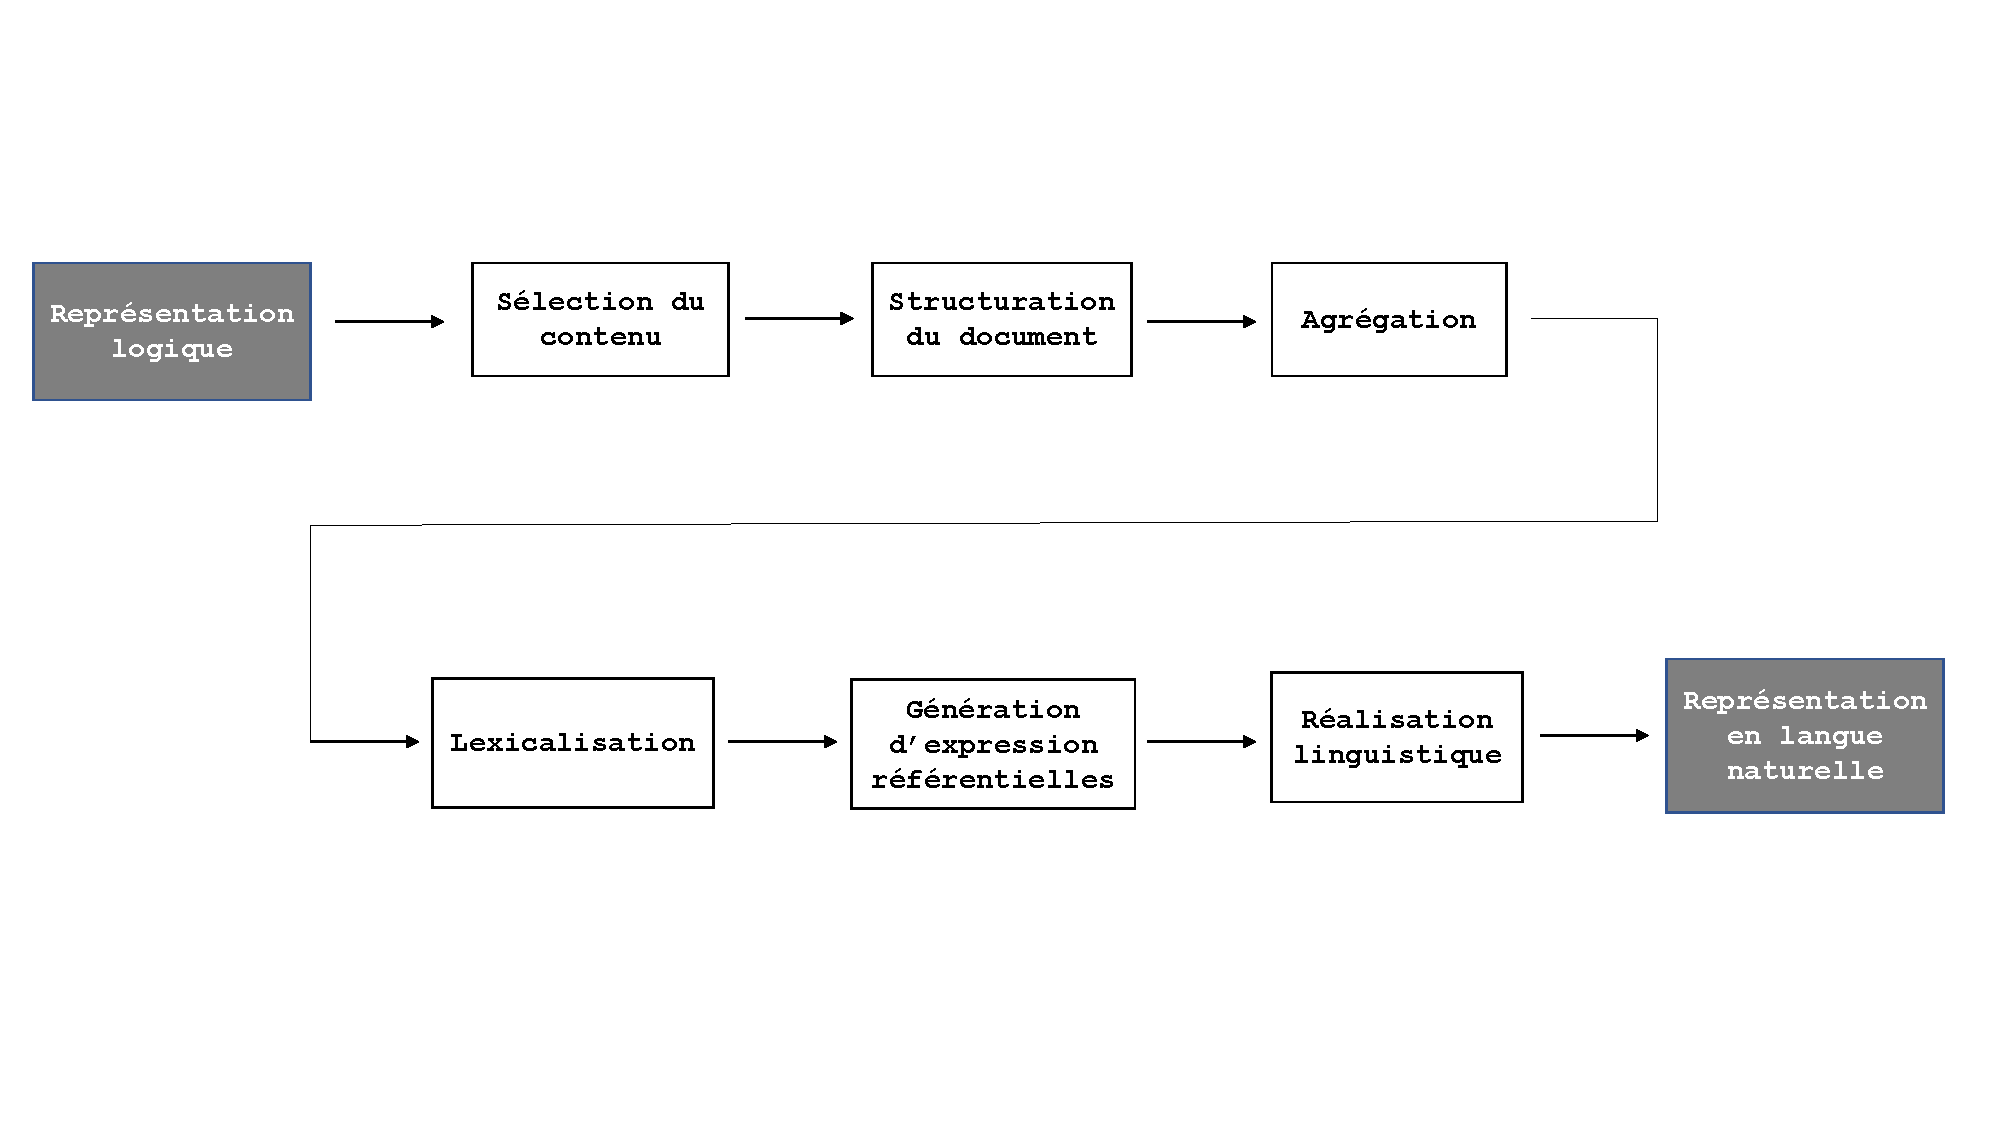
\includegraphics[width=1\textwidth, trim = {0cm 0cm 0cm 0cm},clip]{ch2/figs/pipeline.pdf}
	\caption{Pipeline classique}
	\label{fig:Pipeline}
\end{figure}

\draft{reformuler ce paragraphe}Beaucoup s'entendent pour dire qu'il y a deux parties à la \ac{GAT}. Le \emph{quoi-dire} et le \emph{comment-le-dire} selon \citep{DanlosPresentationmodelegeneration1983}, puis le \emph{early process} et le \emph{late process} selon \citep{gatt18}. Le quoi-dire correspond au early process et le comment-le-dire fait référence au late process. La premier fait référence à la sélection du contenu,la structuration de celle-ci et l'agrégation, puis le second fait référence à toutes les étapes subséquentes : la lexicalisation, la génération d'expressions référentielles et la réalisation linguistique. Pour mieux comprendre le processus de \ac{GAT}, nous décrirons en quelques lignes chacune des étapes qui la compose.

\subsection{Sélection du contenu}
Un système de \ac{GAT} doit départir les informations qui figureront dans le texte de celles qui n'y seront pas. La sélection du contenu dépend de l'objectif de la tâche. Par exemple, si un texte s'adresse à un débutant le niveau de détails du contenu à rendre devra correspondre à l'utilisateur. Il faut donc faire des choix quand au contenu qui sera généré. Par exemple, s'il s'agit de données pour un match de soccer, on ne voudrait probablement pas réaliser en texte toutes les passes et les fautes commises durant le match même si ces informations figurent dans l'input.

\subsection{Structuration du document}
Après avoir sélectionné le contenu, un système de \ac{GAT} doit décider l'ordre dans lequel les informations sélectionnées seront présentées. Reprenons l'exemple du soccer. En fonctions des données choisies, le texte devrait débuter par les informations générales liées au match (où et quand le match s'est déroulé), suivi du noms des équipes qui s'opposaient, puis des points important en terminant par l'issue du match. Il s'agit de créer le plan du texte. Cette étape est une représentation ordonnée et structurée de messages à transmettre. 

\subsection{Agrégation}
L'agrégation est l'étape où on combine des messages en une seule phrase afin de rendre le texte plus fluide et agréable à lire. Les messages sélectionnés dans le plan (structuration du document) n'ont pas à être exprimé dans des phrases individuelles si on peut les combiner en une phrase \citep{ChengCapturingInteractionAggregation2000}. Bref, cette étape sert à rendre le texte moins redondant.

\subsection{Lexicalisation}
À cette étape, une bonne partie de la pré-production a été entamée, on peut commencer à traduire les données non-linguistiques en langue naturelle. Cette partie est très importante car on y sélectionne les mots qui seront utilisés pour transmettre le message. Comme il existe naturellement plusieurs manières pour traduire une même idée en mots, cette tâche peut devenir assez complexe si on veut que le système puisse tenir compte de la réalité du langage. La sélection des mots peut ainsi se faire à divers niveaux d'abstractions. Un niveau plus abstrait requière plus de travail et est plus complexe à mettre en place, mais génère plus de possiblités au moment de la réalisation. Elhadad \cite{ElhadadFloatingConstraintsLexical1997} postulait dès le début une approche en faveur de la lexicalisation profonde.

\subsection{Génération d'expressions réferentielles}
Cette opération est très similaire à la lexicalisation car on choisit comment se réaliseront certaines entités. On l'appelle "`l'étape discriminatoire"' car le but est de s'assurer que le lecteur puisse distinguer correctement chaque entité se trouvant dans le texte. Pour cela, il faut trouver la meilleure façon de référer à une entité.

\subsection{Réalisation linguistique}\label{real}
La dernière étape est la réalisation linguistique. Lorsque tous les mots ont été choisis, puis successivement, toutes les phrases ont été planifiées, il faut les réaliser en texte final et grammatical. Cette tâche implique l'application de traits morpho-syntaxiques aux lexèmes et la linéarisation des structures. Elle inclut aussi l'insertion des mots fonctionnels (auxiliaires, déterminants,etc.) et la ponctuation.

À ce sujet, il existe plusieurs approches pour effectuer la réalisation linguistique. Nous les présentons brièvement ici.

\subsubsection{À base de patrons}
Cette approche est utilisée pour générer du texte dans des domaines précis (météo,sport) et dans lesquels les variations linguistiques réalisables sont minimisées \citep{mcroy_channarukul_ali_2003}. Les phrases en \ref{template} provenant de \cite{gatt18} démontrent comment les patrons s'utilisent.

\ex. \label{template} \emph{À base de patrons}
	\a.\$player scored for \$team in the \$minute minute. 
	\b. Ivan Rakitic scored for Barcelona in the 4th minute.

En \ref{template}, le patron contient trois variables marquées par les \$. Celles-ci peuvent être respectivement comblées par un nom de joueur, suivi d'un nom d'équipe et d'une indication temporelle. Cet exemple démontre bien l'avantage d'utiliser des réalisateurs à base de patrons. Ils permettent de prévoir ce qui sera généré en output et cela diminue les risques d'erreurs. Toutefois, puisqu'ils sont codés à la main, ces sytèmes ont l'inconvénient d'être coûteux en termes de temps. Les réalisateurs à base de patrons peuvent être complémentés par des règles de grammaire, ce qui les rend plus flexibles. Ils peuvent aussi être combinés à de l'apprentissage machine. Cela automatise l'écriture des patrons et rend la tâche moins coûteuse en termes de temps \citep{gatt18}.

\subsubsection{À base de règles grammaticales}
Les modèles à base de règles grammaticales s'emploient autant des les domaines spécifiques (météo, sport) que les domaines généraux (le parler quotidien). Effectivement, ils se prêtent bien à la réalisation de domaine général car ils ont comme fonction de pouvoir réaliser du texte de la manière la plus humaine et naturelle possible. La combinaison de règles de grammaire et de dictionnaires mèneront à la bonne formation de phrases. Cependant, les grammaires et dictionnaires sont codés manuellement, ce qui demande du temps et des ressources.

\subsubsection{Statistiques}
\draft{relire}Il existe divers emplois des méthodes statistiques. On peut l'utiliser pour filtrer les ouputs dans un système où les statisitques détermineront quel output est le meilleur candidat \citep{LangkildeForestbasedStatisticalSentence2000}, approche \emph{generate-and-filter}. Dans cette approche on utilise encore un noyau de règles manuellement encodées. Toutefois, il existe aussi des approches statistiques de réalisation n'utilisant pas de noyau de règles manuellement encodés. Les règles sont apprises automatiquement par apprentissage machine avec de large corpus (white et rajkumar 2012). Cela diminue considérablement la charge de travail manuelle.

\subsubsection{Règles versus statistiques : avantages/inconvénients}

\draft{relire}Maintenant que nous avons présenté ces approches, nous nous posons la question:"' Est-ce que l'encodage manuel est toujours pertinent à l'ère des méthodes statistiques"'. Traditionnellement, les systèmes de \ac{GAT} tendaient vers des ressources encodées manuellement. Mais, de tels ressources nécessitaient du temps (et des ressources). Cela a poussé plusieurs chercheurs à automatiser la réalisation linguistique \citep{LangkildeForestbasedStatisticalSentence2000}.\cite{BelzSystemBuildingCost2009} s'est penché sur cette question dans son article. Concrètement, elle se demandait si le temps qu'on gagne en automatisant la réalisation se fait au détriment de la qualité de celle-ci. Si c'est le cas, à quel point la qualité de l'output est affectée. Elle a évalué une tâche de réalisation en utilisant un système à base de règles, puis un système statistique. L'évaluation se faisait en deux temps. D'abord une évaluation humaine pour traiter la qualité des outputs des deux systèmes, puis une évaluation métrique faite. Après l'évaluation, Belz nous explique que les évaluations humaines pointaient en faveur des systèmes à base de règles. De plus, elle suggère que certaines évaluations métriques surévaluent parfois les systèmes statistiques et sous-évalue les systèmes manuels\citep{BelzSystemBuildingCost2009}. 

\draft{relire}Reiter s'est aussi penché sur la question et il fait un survol du sujet dans son blog \cite{ReiterNaturalLanguageGeneration2016} \draft{vérifier comment citer un blog}. Selon lui, même si les systèmes d'apprentissage machine génèrent du bon texte la plupart du temps, ils peuvent occasionnellement générer du texte bizarre et inapproprié (et les évaluations sont souvent basés sur la moyenne du bon texte généré et pas par rapport aux incongruités générées). De plus, il souligne que lorsque des incongruités sont générées, les systèmes basés sur des méthodes statistiques ont plus de difficultés à les corriger car le tout est basé sur les statistiques. En contre partie, les systèmes à base de règles où permettent de cerner le problème avec plus de facilité et le corriger. Ce comportement n'est pas approprié dans des domaines professionnels ou personnels où des utilisateurs comptent sur la qualité des textes générés automatiquement, entre autre, car ils prendront potentiellement des décisions en fonction de leur lecture. Cependant, Reiter termine son article de blog en soulignant que la \ac{GAT} a beaucoup à gagner des méthodes statistiques. Il suggère de se servir de celles-ci pour automatiser des composantes d'une approche à base de règles.

%%%%%%%%%%%%%%%%%%%%%%%%%%%%%%%%%%%%%%%%%%%%%%%%%%%%%%%
% --------- R É A L I S A T I O N   ---------
%%%%%%%%%%%%%%%%%%%%%%%%%%%%%%%%%%%%%%%%%%%%%%%%%%%%%%%


\section{Réalisation}

Notre projet concerne strictement la réalisation. C'est pourquoi, pour une meilleure compréhension de cette étape du processus de \ac{GAT}, nous décrirons quelques réalisateurs brièvement.

Tel qu'explicité à la figure~\ref{fig:Pipeline}, la réalisation est la dernière étape dans le processus de \ac{GAT}. Toutefois, pour beaucoup de chercheurs, elle ne représente pas uniquement les tâches décrites précédemment. Il règne une ambiguité quant aux concepts qu'incarne la réalisation. Pour certains, la réalisation correspond exactement à ce qu'on a présenté dans la section \ref{real}. On appellera cela la réalisation de surface, puisque la réalisation se fait à partir d'un input beaucoup plus près du texte. Notamment des structures syntaxiques lexicalisées. Pour d'autres, la réalisation se fait à partir de données plus abstraites et contient la lexicalisation. Autrement dit, au moment de la réalisation, la lexicalisation n'a pas été effectuée encore. Elle prend généralement en input non-syntaxiques. On les appellera des réalisateurs profonds. Les informations lexicales et grammaticales seront encodées dans des dictionnaires et des grammaires plus complexes permettant de traiter l'interace sémantique-syntaxe. Finalement, ces systèmes profonds sont généralement liés à une théorie linguistique leur permettant de modéliser le langage et de l'encoder dans un système informatique.

%%%%%%%%%%%%%%%%%%%%%%%%%%%%%%%%%%%%%%%%%%%%%%%%%%%%%%%
% --------- R É A L I S A T E U R   S U R F A C E ---
%%%%%%%%%%%%%%%%%%%%%%%%%%%%%%%%%%%%%%%%%%%%%%%%%%%%%%%

\subsection{Réalisateurs de surface}

Dans cette section, nous vous présenterons quelques réalisateurs de surface. En commençant par SimpleNLG, puis JSreal et finalement RealPro.

\subsubsection{SimpleNLG}
SimpleNLG est \citep{GattSimpleNLGRealisationEngine2009} est un réalisateur de surface écrit en java. Le texte est réalisé à partir d'une structure syntaxique déjà lexicalisée encodée en XML. Par la suite, le réalisateur opère les opérations morphologiques nécessaires (flexion, dérivation des mots, linéarisation, ajout d'auxiliaires, gestion de l'accord) tout en linéarisant le texte.

Puisqu'il s'agit d'un réalisateur à base de règles, SimpleNLG est évidemment doté d'une grammaire et d'un dictionnaire. Ce dernier encode les propriétés syntaxiques et morphologiques des unités lexicales. Tandis que le module grammatical contient des règles permettant le passage de la syntaxe à la morphologie.

SimpleNLG découpe son processus de réalisation en quatre. Premièrement, les lexèmes compris dans la structure d'input sont mis en correspondance avec leur entrée de dictionnaire. Deuxièmement, \draft{me manque la deuxième étape}. Troisièmement, on combine les lexèmes en fonction de la structure et on crée des syntagmes de plus en plus large, jusqu'à ce que l'entièreté de la phrase forme un syntagme phrastique. Finalement, celui-ci est linéarisé puis les lexèmes sont accordés en fonction des règles morphologiques pour obtenir les formes fléchies.

\draft{mettre les citations dans references.bib}Noter que SimpleNLG a été traduit dans plusieurs langues : espagnol, italien, et français, portugais (Mazzei et al., 2016, Ramos-Soto 2017, Vaudry et Lapalme 2013 ; Oliveira et Sripada)

\begin{lstlisting}[language=Xml, caption=Structure d'input dans SimpleNLG, label=simplenlg]
<Document>
  <child xsi:type="SPhraseSpec">
    <subj xsi:type="VPPhraseSpec" FORM="PRESENT_PARTICIPLE">
      <head cat="VERB">
        <base>refactor</base>
      </head>
    </subj>
    <vp xsi:type="VPPhraseSpec" TENSE="PRESENT" >
      <head cat="VERB">
        <base>be</base>
      </head>
      <compl xsi:type="VPPhraseSpec" FORM="PAST_PARTICIPLE">
        <head cat="VERB">
          <base>need</base>
        </head>
      </compl>
    </vp>
  </child>
</Document>
\end{lstlisting}
\draft{utiliser les formats de descriptions de phrase TST}La figure \ref{simplenlg} permet de réaliser la phrase 'Refactoring is needed.'

\subsubsection{JSreal}
JSreal \citep{DaoustJSREALTextRealizer2015} qui signifie JavaScript Realiser est un réaliseur de texte orienté pour les programmeurs web. Il génère des expressions et phrases bien formées qui peuvent être formattées en HTML pour être exposé dans un fureteur. Il peut aussi s'employer seul à des fins purement linguistiques et être intégéré dans des générateurs de textes automatiques. En règles générales, les spécificités de JSreal sont assez similaires à celles de SimpleNLG \citep{GattSimpleNLGRealisationEngine2009}.

Pour générer du texte JSreal prend en input des structures syntaxiques lexicalisées. La construction de la phrase découle de l'application de règles syntaxiques et morphologiques déclenchées par les lexèmes dans les structures syntaxiques. JSreal fonctionne autour des modules suivants : un dictionnaire et une grammaire. Son dictionnaire défini la catégorie des mots qui le peuple, et les traits lexicaux qui leurs sont attachés (genre, nombre, irrégularités, etc.). La grammaire contient des règles morpho-syntaxiques qui permettent de faire l'accord entre les constituants correctement. Finalement, il existe aussi une version bilingue de JSreal \citep{MolinsJSrealBBilingualText2015} qui incorpore le français et l'anglais.

\begin{lstlisting}[language=Xml, caption=JSreal, label=jsreal]
JSrealLoader({
        language: "en",
        lexiconUrl: URL.lexicon.en,
        ruleUrl: URL.rule.en,
        featureUrl: URL.feature
    }, function() {
    QUnit.test( "Sentence EN", function( assert ) {
        assert.equal(
            S(
                NP(D("the"), N("cat")),
                VP(V("sit"), PP(P("on"), NP(D("the"), N("coach")))).t("ps")
            )
        
\end{lstlisting}
\draft{Présenter la phrase correctement en TST}La figure \ref{jsreal} produit la phrase :'The cat sat on the coach.'
		
\subsubsection{RealPro}
RealPro est implémenté en C++ \citep{LavoieFastPortableRealizer1997}. Il est le plus profond des réalisateurs de surface préséntés jusqu'ici. Il prend en input des arbres de dépendances, ce qui le distingue des inputs présentés jusqu'ici \citep{DaoustJSREALTextRealizer2015},\citep{GattSimpleNLGRealisationEngine2009}.L'architecture de RealPro est basé sur la TST \citep{melcuk1988}. Brièvement, il s'agit d'une théorie qui divise le langage en divers niveaux de représentations. Le niveau le plus abstrait étant la sémantique, puis la syntaxe,  suivie de la morphologie , et de la parole (ou du texte dans ce contexte). Ainsi, ce système part aussi d'une représentation syntaxique, mais d'une représentation syntaxique profonde et de dépendance. \draft{expliquer brièvement ce qu'est un arbre de dépendance}

La première étape à effectuer pour éventuellement se rendre à l'output désiré est le passage syntaxe profonde à celle de surface. Pour ce faire, le logiciel effectue la transition en passant par son dictionnaire et ses règles de grammaires pour s'assurer que le passage soit grammatical. Il en va de même pour toutes les transitions successives : de la syntaxe de surface à la morphologie profonde, jusqu'à la morphologie de surface, jusqu'au texte final. Ainsi, les modules dictionnairiques et grammaticaux sont réquisitionnés par les diverses composantes du réalisateur au cours de la génération. Le graphique \ref{fig:RealPro} démontre leurs intéractions lors de la réalisation.
\begin{figure}[htb]
	\centering
	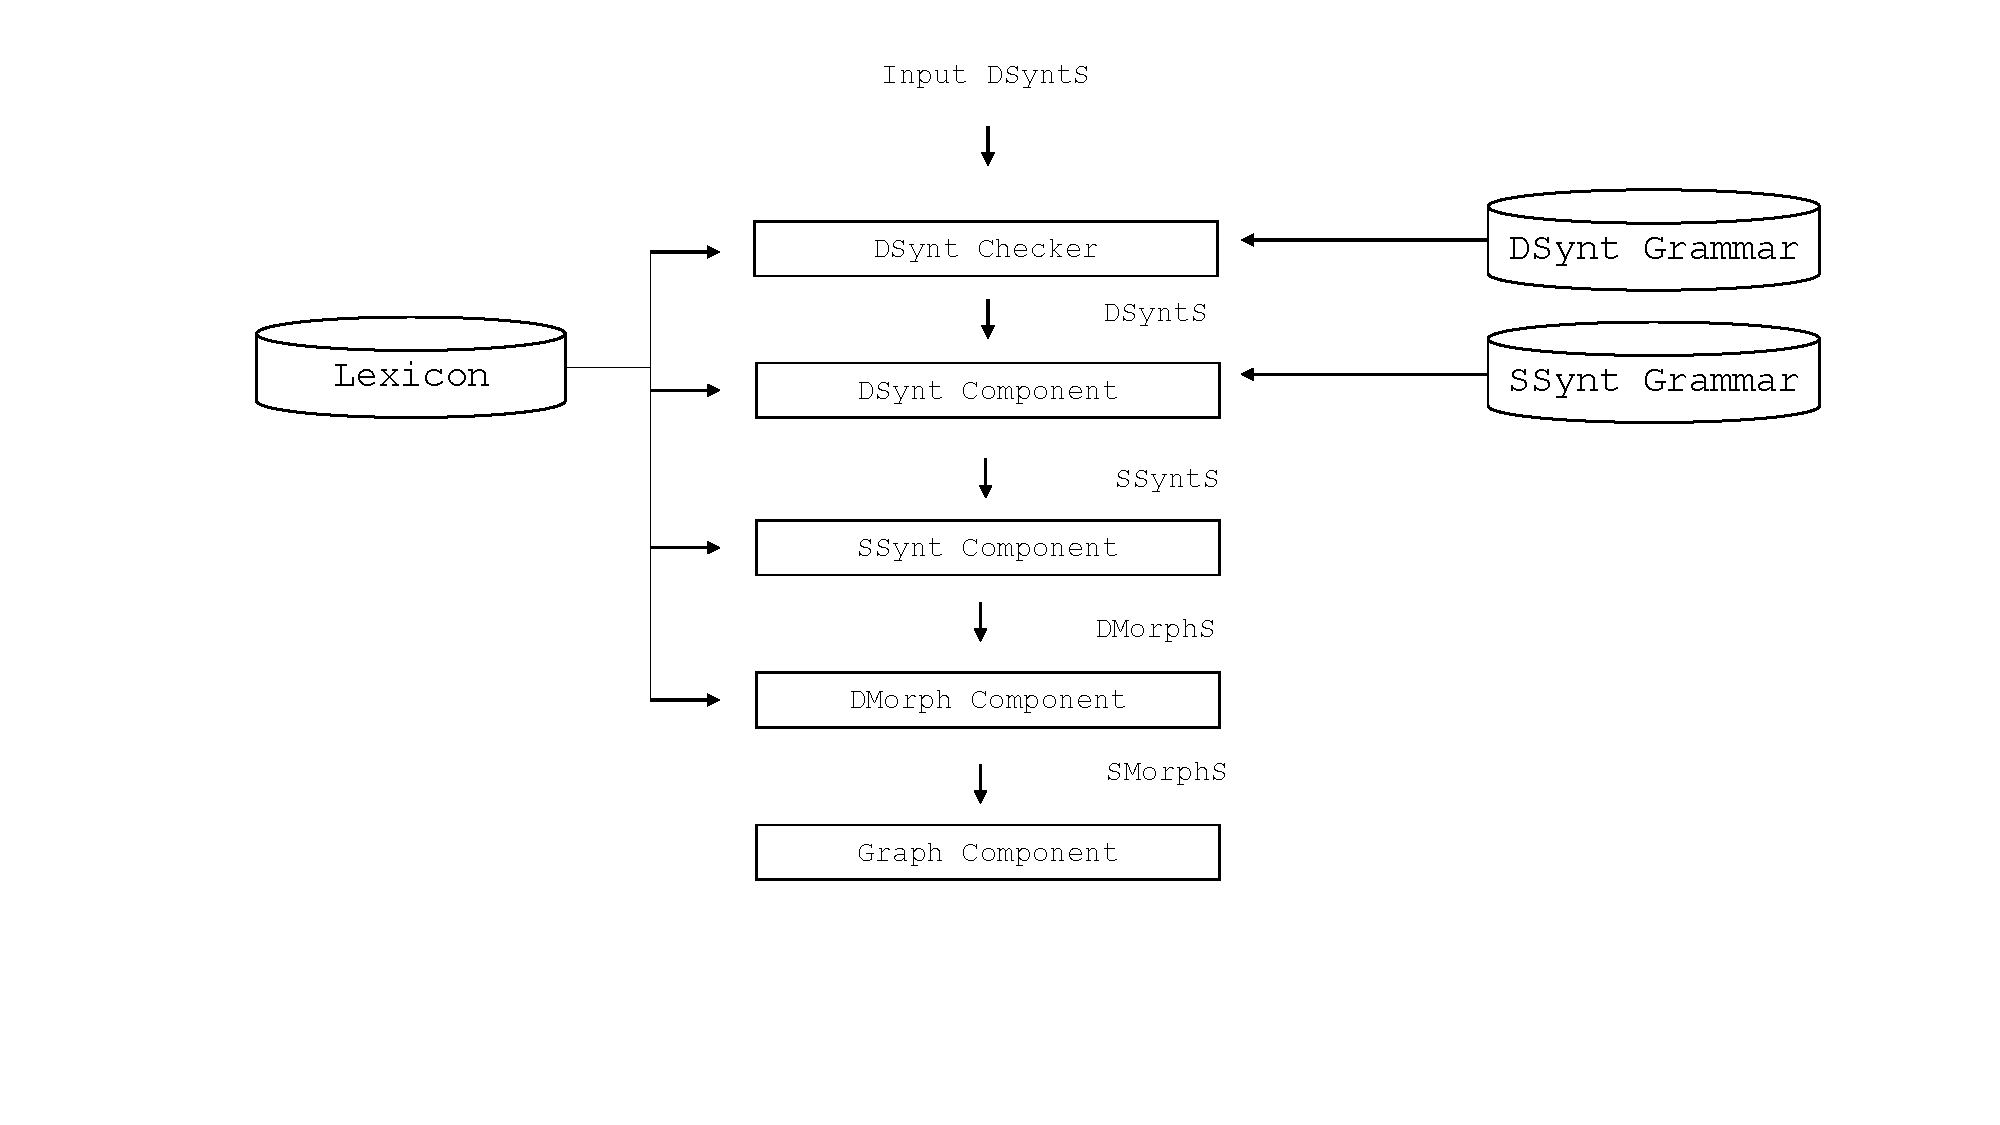
\includegraphics[width=1\textwidth, trim = {0cm 0cm 0cm 0cm},clip]{ch2/figs/realpro.pdf}
	\caption{RealPro}
	\label{fig:RealPro}
\end{figure}

Voici à quoi ressemble un input pour ce système. La figure \ref{realpro} est un arbre de dépendance représentant la phrase \draft{changer le format de l'exemple} 'March had some rain days.'
\begin{lstlisting}[language=Xml, caption=Input, label=realpro]
HAVE1 [tense:past]
(I March [class:proper-noun]
II day [class:common-noun numberpl]
(ATTR rainy [class:adjective]))
\end{lstlisting}


%%%%%%%%%%%%%%%%%%%%%%%%%%%%%%%%%%%%%%%%%%%%%%%%%%%%%%%
% --------- R É A L I S A T E U R    P R O F O N D  ---
%%%%%%%%%%%%%%%%%%%%%%%%%%%%%%%%%%%%%%%%%%%%%%%%%%%%%%%

\subsection{Réalisateurs profonds}

Maintenant que nous avons exposé quelques générateurs de surface, nous présenterons quelques réalisateurs profonds. Ceux-ci prennent généralement en input des structures plus abstraites entraînant une plus grande flexibilité linguistique dans le contenu généré. Les réalisateurs profonds incorporent généralement la lexicalisation, ce qui fait en sorte que les concepts à réaliser ne sont pas encore fixés et c'est là que la flexibilité entre en jeu \citep{PolguerePourmodelestratifie}. Effectivement, on laisse place au paraphrasage puisqu'une même idée peut être exprimée de différentes manières. Dans le pipeline classique, comme nous l'avons vu, la lexicalisation est opérée avant la réalisation. Cela fait en sorte que les inputs contiennent déjà des lexèmes et cela restreint grandement les réalisations possibles puisque les lexèmes incorporent des combinaitoires bien précises et la phrase à générer doit s'articuler autour de ces contraintes. 

Nous présenterons les réalisateurs profonds suivants: KPML, Surge, FORGe et MARQUIS.

\subsubsection{KPML}
KMPL\citep{BatemanEnablingTechnologyMultilingual1997} est un réalisateur multilingue héritier du système PENMAN \citep{PenmanOverview}. La théorie linguistique sous-jacente à ce système est la \acf{SFG} \citep{MatthiessenSystemicfunctionalgrammar1997}. Cette théorie postule que les choix linguistiques sont déclenchés par l'exécution d'une fonction. D'un point de vue multilingue, les différentes langues issues de KPML partagent un grand nombre de fonctions, puis quelques fonctions. Autrement dit, dans ce formalisme, la forme de surface est la conséquence directe de la sélection d'un ensemble de traits fonctionnels abstraits à partir des réseaux systémiques. Dans ce formalisme, la réalisation linguistique se fait en traversant les réseaux.La grammaire de ce système est implémentée à la manière d'un réseau de système orienté qu'on lit de gauche à droite. Les intersections dans le réseau correspondent à un choix grammatical à faire entre différents traits fonctionnels. Ces choix grammaticaux deviennent de plus en plus pointus à force qu'on avance dans le réseau. Finalement, cette grammaire incorpore tous les aspects linguistiques: sémantique, syntaxe, morphologie, etc.

Les informations comprises dans les inputs de ce système sont d'ordre sémantiques et syntaxiques. Plus précisément, KPML prend des \acf{SPL} en entrée. Un \ac{SPL} est une matrice dont les objets sont des paires d'attributs et de valeurs. Afin d'illustrer à quoi ressemble l'input, nous vous présentons la figure \ref{kpml} qui provient de \cite{ReiterBuildingNaturalLanguage2000} \draft{mettre la phrase dans le bon format: 'March had some rainy days'.}
\begin{lstlisting}[language=Xml, caption=SPL: input de KPML, label=kpml]
(S1 \ generalized-possession
  :tense past 
	:domain (N1 \ time-interval
	            :lex march
							:determiner zero)
	:range (N2 \ time-interval
	           :number plural
						 :lex day
						 :determiner some
						 :property ascription
						 (A1 \ quality :lex rainy)))
\end{lstlisting}

\subsubsection{Surge}
Surge, qui signifie \emph{Systemic Unification Realisation Grammar of English}, est une grammaire de l'anglais\citep{Elhadad98surge:a}. Elle est écrite en \acf{FUF} qui est basé sur \acf{FUG} \citep{KayFunctionalUnificationGrammar1984}. \ac{FUF} est un langage de programmation créé pour construire des grammaires computationnelles, plus particulièrement pour les besoins de la réalisation dans un cadre de grammaire d'unification. \draft{comprends pas comment fonctionne la grammaire FUF- dois lire là-dessus}

Une grammaire \ac{FUF} prend en entrée des \acf{FD}. Celles-ci décrivent à la fois le sens d'une phrase et la grammaire. Celle-ci est aussi décrite en termes de descriptions fonctionnelles. Celles sont aussi des matrices de paire d'attributs et de valeurs dont l'union fournit une spécification de l'énoncé à génerer. \ac{FUF} génère en output une phrase exprimant le sens voulu et suivant les règles de la grammaire.Contrairement aux autres réalisateurs présentés ici, le modèle \ac{FUF} n'utilise pas de dictionnaires. L'information lexicale est encodée dans la structure d'input \ref{surge}.

Dans Surge, la réalisation se fait en deux temps. D'abord, on procède à l'unification des \ac{FD} du sens de la phrase à réaliser. Autrement dit, on enrichie la structure d’entrée avec les spécifications syntaxiques et morphologiques de la grammaire. Puis, \ac{FUF} effectue la linéarisation de la structure afin de réaliser la phrase et les contraintes morpho-syntaxiques sont opérées (l'accord, les constructions syntaxiques, etc.)

Nous reprendrons encore un exemple tiré de Dale et Reiter \cite{ReiterBuildingNaturalLanguage2000} \draft{mettre la phrase dans le bon format: 'March had some rainy days'.}
\begin{lstlisting}[language=Xml, caption=FD: input de Surge, label=surge]
((cat clause)
 (proc ((type possessive)))
 (tense past)
 (partic ((possessor ((cat proper) head ((lex "March"))))
					(possessed ((cat common) head ((lex day)))
											(describer ((lex rainy)))
											(selective yes) (number plural)))))
\end{lstlisting}

\subsubsection{FORGe}
FORGe est un transducteur de graphes qui génère du texte à l'aide de ressources lexicales dictionnairiques et grammaticales \citep{MilledemoFORGePompeu2017},\citep{DBLP:conf/semeval/MilleCBW17}. C'est un réalisateur profond qui a hérité de l'architecture de MARQUIS \citep{WannerMARQUISGENERATIONUSERTAILORED2010}. Nous décrirons cet autre réalisateur à la section \ref{sectionmarquis}. FORGe a été conçu pour l'anglais à la base, mais il se veut multilingue (espagnol, allemand, français et polonais sont en développement). C'est un réalisateur qui peut aisément générer du texte en différentes langues grâce à ses règles grammaticales qui sont majoritairement \emph{language-independent}. Les autres règles qui sont propres à l'anglais peuvent aisément être adaptées à d'autres langues.

La théorie linguistique sous-jacente à ce système est la théorie Sens-Texte \draft{mettre un livre sur la TST en citation}. D'ailleurs nous verrons plus en détails dans la section \ref{chapgendr} au chapitre suivant comment cette théorie linguistique se prête à transducteur de graphes. Pour l'instant nous en traiterons dans les grandes lignes.

En ce qui concerne le réalisateur FORGe, il prend en input des représentations sémantiques en graphes acycliques. Ceux-ci sont composés de relations liant des arguments à des prédicats. Pour visualiser de quoi on parle, ce type de graphe correspond à la structure \#2 dans la figure \ref{fig:marquis} dans la section MARQUIS \ref{sectionmarquis}. Donc FORGe est un réalisateur profond car il prend en input une structure sémantique dépourvue de syntaxe et dont les unités sont de types sémantiques et non lexicales.

La réalisation de texte dans FORGe se découpe en trois étapes : le transfert de la RSem à la RSyntP, suivi du transfert de la RSyntP à la RSyntS, et finalement de la RSyntS au texte linéarisé et morphologisé. 

Le passage de la représentation sémantique à la structure syntaxique profonde est effectuée via un parsing récursif \emph{top-down}. Le top est la racine de l'arbre de dépendance en développement. (on crée un noeud vide, mais avec des contraintes) ,on vérifie que le lexème qui consommera le noeud correspond à la partie du discours requise par ce noeud. Une fois que le top est lexicalisé en syntaxe (avec un lexème qui respecte les contraintes), on crée de nouvelles branches partant de la racine. Ces branches correspondent aux noeuds des dépendants syntaxiques de la racine. Ensuite, on cherche dans le dictionnaire une entrée lexicale qui correspond au sens correspondant (dans le graphe sémantique) et qui satisfait les contraintes. Puis une fois que ces noeuds sont lexicalisés, on répète la tâche précédente et ainsi de suite jusqu'à ce qu'on ait parsé la représentation sémantique au complet. Le résultat final est un arbre de dépendance lexicalisé correspondant au graphe en entrée. Pour que le tout se fasse correctement, le système utilise une combinaison de règles de grammaire et des dictionnaires.L'opération est effectuée successivement jusqu'à ce que toute la représentation sémantique ait été analysée.

Le passage de la syntaxe profonde à la syntaxe de surface correspond à l'étape où on introduit les mots fonctionnels(prépositions, auxiliaires, déterminants) et les relations de surface (sujet, objet direct, etc.) dans l'arbre de dépendance. Cette étape est possible grâce à la complexité des dictionnaires que FORGe utilise. Puisque les verbes sont très variés et que les prépositions requises dans certains contextes diffèrent d'un verbe à un autre, il faut que ces infos soient encodées quelque part. Ils ont eu l'idée de créer un dictionnaire où la valence des verbes y seraient répertoriés et cela permettrait une encore plus grande flexibilité au système pour tenir compte des particularités des langues. Nous reviendrons à cette problématique dans la section problématique \ref{problema} au chapitre suivant \ref{chapgendr}.

Finalement, la dernière étape de ce réalisateur consiste à appliquer les règles morpho-syntaxiques aux lexèmes et à linéariser la structure syntaxique de surface pour en générer un texte final.

\subsubsection{MARQUIS}\label{sectionmarquis}

Contrairement aux autres systèmes présentés ici, MARQUIS n'est pas qu'un réalisateur profond. Il s'agit d'un système de \ac{GAT} complet qui effectue toutes les étapes du processus de génération automatique de texte (section \ref{ppc}). Cependant, nous ne nous intéresserons qu'à son aspect de réalisation profonde. Pour plus d'informations, nous vous réferons à l'article \citep{WannerMARQUISGENERATIONUSERTAILORED2010}. 

Le but du projet MARQUIS est de générer, à partir de données brutes, des bulletins météorologiques multilingues sur la qualité de l'air. Ces bulletins sont générés en fonction de l'utilisateur. Ainsi, une personne doit entrer ses informations personnelles dans le module de l'utilisateur, puis le bulletin sera générée, par exemple, en fonction de son expertise ou de sa condition physique (problèmes respiratoires, etc.).

MARQUIS est aussi un système basé sur la Théorie Sens-Texte, comme FORGe \citep{MilledemoFORGePompeu2017} et RealPro \citep{LavoieFastPortableRealizer1997}. La réalisation profonde se fait sensiblement avec les mêmes mécanismes que FORGe, mais elle compte un niveau de profondeur de plus: représentation conceptuelle. Effectivement, MARQUIS étant un générateur multilingue (l'anglais, l'allemand, l'espagnol, le catalan, le portugais, le français, le finnois et le polonais.), le niveau de profondeur commun à toutes les langues du système et le niveau conceptuel. Celui-ci est encodé en graphes conceptuels et il forme un interface conceptuelle-sémantique avec le niveau sémantique. L'étape de réalisation profonde est ainsi la même que nous avons décrit avec FORGe, avec la particularité que MARQUIS ne fait pas appel à un dictionnaire de valence (il a donc moins de couverture). Afin de mieux expliciter la chose, la figure \ref{marquis} démontre bien comment ce système fonctionne.

MARQUIS part de la représentation conceptuelle qui passe par les niveaux de représentations jusqu'au texte.

\begin{figure}[htb]
	\centering
	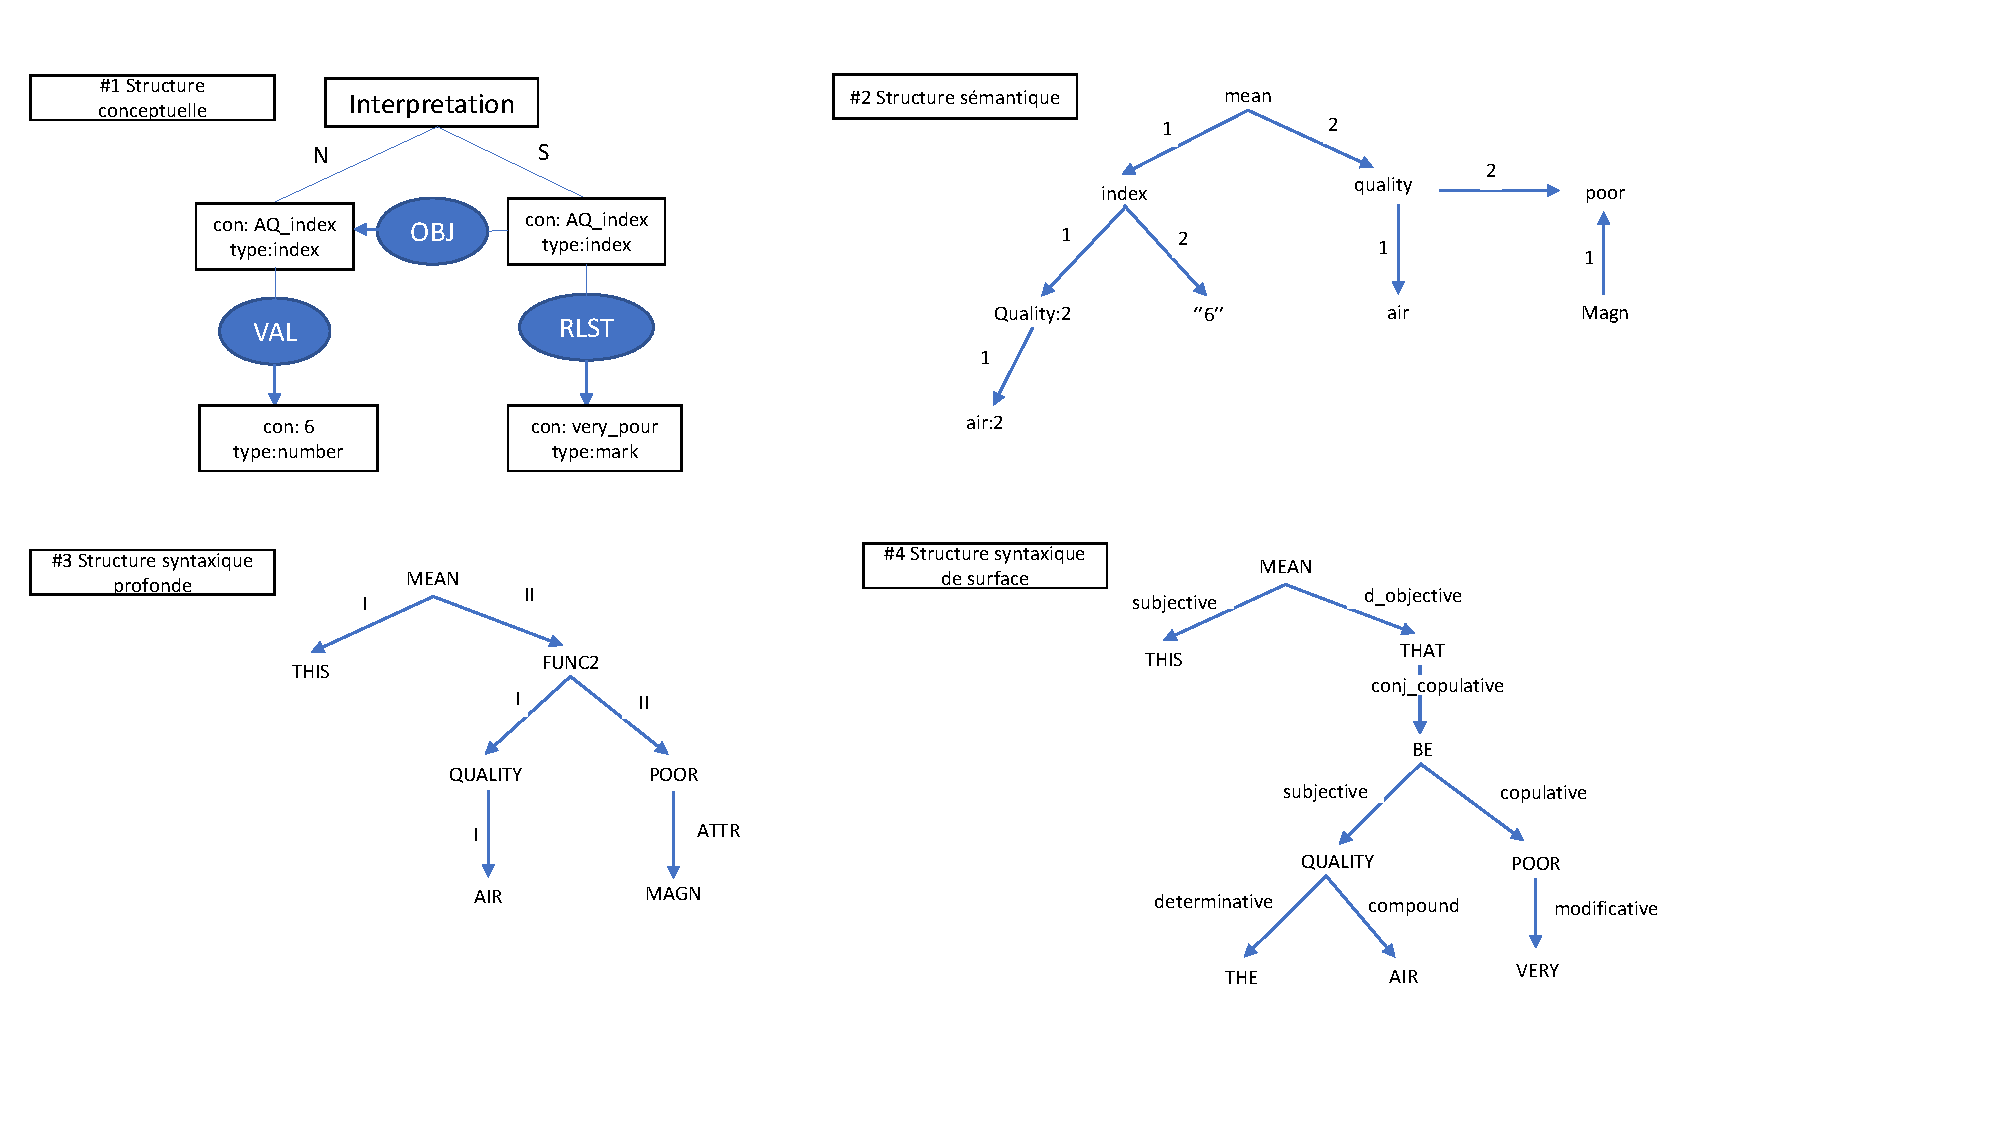
\includegraphics[width=1\textwidth, trim = {0cm 0cm 0cm 0cm},clip]{ch2/figs/marquis.pdf}
	\caption{Pipeline de MARQUIS}
	\label{fig:marquis}
\end{figure}

Pour résumé cette figure
Prend en input : graphes conceptuels 
rend en output : du texte
entre les 2 : séries de dérivations (changements successifs de représentations en fonction des divers niveaux de représentations. ce qui assure la grammaticalité des changements est : l'information lexicale encodée dans les dictionnaires et les modules de règles qui modélise chaque interface).

Par exemple, voici comment les dictionnaires et règles fonctionnent \draft{reprendre la figure 11 de Florie}
Le dictionnaire conceptuel comprend tous les concepts utiles à la génération des rapports sur la qualité de l'air et les autres termes généraux du langage. Puis il mappe les concepts aux unités sémantiques (dans chaque langue) qui leurs correspondent. Le dictionnaire sémantique contient les unités sémantiques. Une même unité sémantique peut être réalisée par deux lexèmes différents. Ainsi, il nous faut un dictionnaire lexémique qui contient toutes les unités lexicales et leurs traits. Par la suite, une fois que les unités sont lexicalisées, nous n'avons plus besoin d'autres dictionnaires. 

Tel que démontré, MARQUIS et FORGe partent de niveaux d'abstraction plus profond que les autres systèmes présentés. Cela leur permet d'être beaucoup plus flexible dans leur réalisation linguistique. C'est pourquoi nous utilisons aussi un réalisateur profond doté de paramètres très similaires à ces deux réalisateurs. Comme FORGe, nous utiliserons aussi un système basé sur MARQUIS. Il s'agit de GenDR \citep{lareau18}: un projet en cours de développement dirigé par François Lareau à l’Observatoire de linguistique Sens-Texte. Le chapitre suivant décrira en détails ce réalisateur.